\documentclass[12pt]{article}
\title{EE445M Lab 4}
\author{Hershal Bhave (hb6279) and Eric Crosson (esc625)}
\date{Friday April 03, 2015}

\usepackage[in]{fullpage}
\usepackage{listings}
\usepackage{tabularx}
\usepackage{cleveref}
\usepackage[nosolutionfiles]{answers}
\usepackage{graphicx}
\usepackage{xcolor}
\usepackage{color}
\usepackage{enumerate}
\usepackage{pdfpages}
\usepackage{float}
\usepackage{subcaption}

\newenvironment{Ex}{\textbf{Problem}\vspace{.25em}\\}{}
\Newassociation{solution}{Soln}{Answers}
\pagebreak[3]
\newcommand{\Opentesthook}[2]{\Writetofile{#1}{\protect\section{#1: #2}}}
\renewcommand{\Solnlabel}[1]{\textbf{Solution}\quad}
\newcommand{\todo}{{\LARGE \emph{\color{red}TODO}}}
\newcommand{\ohm}{$\Omega$}
\newcommand{\hbr}{\hfill\vspace{.25em}\\}
\newcommand{\dd}[1]{\:\mathrm{d}{#1}}
\newcommand{\ddt}[1]{\frac{\dd{}}{\dd{#1}}}
\newcommand{\dddt}[1]{\frac{\dd{}^2}{\dd{#1}^2}}

\definecolor{mygreen}{rgb}{0,0.6,0}
% \definecolor{mygreen}{rgb}{0.13,0.55,0.13}
\definecolor{mygray}{rgb}{0.5,0.5,0.5}
\definecolor{mymauve}{rgb}{0.58,0,0.82}

\lstset{
  backgroundcolor=\color{white},
  basicstyle=\scriptsize\ttfamily,
  breakatwhitespace=false,
  breaklines=true,
  captionpos=b,
  commentstyle=\color{mygreen},
  deletekeywords={...},
  escapeinside={\%*}{*)},
  extendedchars=true,
  frame=single,
  keywordstyle=\color{blue},
  % language=Octave,
  % numbers=left,
  % numbersep=5pt,
  % numberstyle=\tiny\color{mygray},
  rulecolor=\color{black},
  showspaces=false,
  showstringspaces=false,
  showtabs=false,
  % stepnumber=2,
  stringstyle=\color{mymauve},
  tabsize=2,
  title=\lstname,
  columns=fullflexible,
}

\begin{document}
\maketitle

\section{Objectives}
\begin{itemize}
\item Interface a microphone and record sounds
\item Design and implement an analog HPF, LPF and digital FIR filters
\item Build a spectrum analyzer
\item Write a real-time application that displays in both the time
  domain and the frequency domain
\end{itemize}

\section{Hardware Design}
At the end of this document the reader will find the TI FilterPro
design specification for the low-pass filter used in this lab.

\section{Software Design}
Reference \cref{lst:lab4}. We have distinct functions to handle the
data manipulation and modes of operation. Semaphores guard shared
resources and timers dictate periodic tasks. Users may switch between
modes by entering commands through the shell via UART or by the
onboard buttons.

To facilitate debugging, we found it convenient to monitor operations
in the absence of periodic timer interrupts. In our system, periodic
timers were used to trigger the ADC sampling. Each timer interrupt
triggered the data acquisition process, which interferes with
debugging flow. To allow for seamless debugging, we introduced an ADC
simulator. The method \verb|simulate_adc| iterates over a sine wave in
memory and feeds the sequential values into the FIFO that normally
takes information from the ADC. As such, normal program execution
continues with simulated sinusoids. This mechanism allowed us to test
LCD plotting and the software low-pass filter without a hardware
signal generator.

Each component was tested (plot graphics, data acquisition, filter
accuracy) was done by both visual examination and by comparing the
actual data versus ideal data in Octave.

\section{Measurement Data}
\begin{description}
\item[Dynamic circuit performance] \hbr
  \Cref{fig:oscope-plots} shows the performance of the analog
  low-pass filter at various frequencies. The ideal cutoff frequency
  for our low-pass filter was 500Hz.
\item[Spectrum analyzer data] \hbr
  Absent.
\item[FIR filter test data] \hbr
  \Cref{fig:lcd-plots-raw} includes photographs of the LCD display
  during sampling of the indicated frequency from a signal
  generator. \Cref{fig:lcd-plots-filtered} shows the same frequencies
  as they are run through a software low-pass filter. The axes are
  amplitude vs. time.
\end{description}

\section{Analysis and Discussion}
\begin{enumerate}[1)]
\item
  \begin{Ex}
    How did measured frequency responses compare to your estimations
    of cutoff frequencies for your HPF and LPF?
    \begin{solution} \hbr
      The low-pass filter was created using Octave in the code
      referenced in \cref{lst:filtergen}. TI's FilterPro was used to
      calculate the analog low-pass filter cutoff frequencies. The
      actual low-pass filter cutoff frequency was slightly different
      than the ideal calculated value since we used different resistor
      values (2.2k\ohm resistors compared to FilterPro's recommendation
      of 2.24k\ohm).
    \end{solution}
  \end{Ex}
\item
  \begin{Ex}
    Explain how you measured maximum bandwidth. What was the
    limiting factor affecting bandwidth?
    \begin{solution} \hbr
      \todo since we don't have fft... isn't that going to be the most
      computationally intensive (bandwidth-limiting) section?
    \end{solution}
  \end{Ex}
\item
  \begin{Ex}
    What is the expected FFT output if the input is a square wave?
    \begin{solution} \hbr
      Impulses on the harmonic frequencies of the square wave emerge on
      the frequency vs. apmlitude plot.
    \end{solution}
  \end{Ex}
\item
  \begin{Ex}
    Look at the noise in your digital samples when it is very
    quiet. What noise is this?
    \begin{solution} \hbr
      The noise is error introduced by the sampling components,
      mathematical rounding errors, and timing jitter.
    \end{solution}
  \end{Ex}
\item
  \begin{Ex}
    Can you estimate jitter in your ADC samples?
    \begin{solution} \hbr
      No, we did not implement jitter calculation in this lab. There
      should be little to no jitter, as timers are utlized to provide
      adc triggering and each interrupt service routine takes a
      consisten amount of time regardless of the data the ADC is
      sampling. Care was taken to make sure that the ISRs take an
      equal amount of time for this purpose.
    \end{solution}
  \end{Ex}
\item
  \begin{Ex}
    Prove your FIR implementation can not overflow.
    \begin{solution} \hbr
      Our ADC samples voltages which convert to integer values between
      0 to 4095, inclusive, which is then offset by -2048 to make our
      data fit between -2048 and 2047. Our filter is of length
      51. During our \verb|convolve| function, we multiply and
      accumulate the value from the ADC by the value from the
      filter. In a worst-case scenario, the filter would continuously
      apply \verb|y[i] += (-2048)*(-2048)| 51 times for one index of
      the low-pass filter data. The maximum value possible during this
      calculation is 213909504. The maximum allowable signed 32-bit
      integer value is 2147483648, a difference of 1933574144. Thus,
      it is impossible for our filter to overflow.
    \end{solution}
  \end{Ex}
\item
  \begin{Ex}
    Look at symmetry in the \verb|h[51]| coefficients in the example
    FIR design. How could you rewrite the following filter equation to
    reduce the number of multiplies from 51 to 26?
    $y[i]=(h[0]*x[i]+h[1]*x[i-1]+h[2]*x[i-2]+\cdots+h[50]*x[i-50])/256;$
    \begin{solution} \hbr
      \todo I'm not sure... will revisit.
    \end{solution}
  \end{Ex}
\item
  \begin{Ex}
    Explain how the multiple and accumulate instruction (MLA) can
    reduce the execution time of your filter. If you were to have used
    the MLA instruction, would your filter have been more accurate?

    \begin{solution} \hbr
      MLA obviates the need for adding the products we determine to a
      separate accumulator. Since the accumulator is handled by MLA
      hardware, the amount of transferring bits around the
      microarchitecture at the speed of the bus clock is reduced. Similar
      to tail-chaining of interrupt service vectors, slight hardware
      optimization is provided for this common task.

      Our filter would have been more accurate since \verb|IEEE 754-2008|
      specifies this instruction must be implemented with only one
      rounding (instead of two). This reduces total error accumulation
      over time.
    \end{solution}
  \end{Ex}
\end{enumerate}

\newpage
\section{Figures}

\begin{figure}[H]
  \centering
  \begin{subfigure}[b]{0.3\textwidth}
    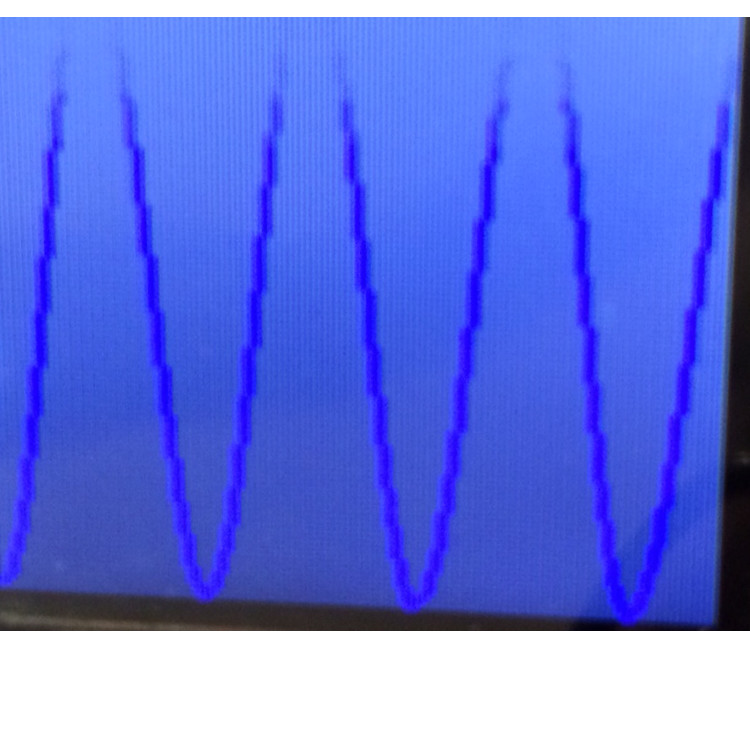
\includegraphics[width=\textwidth]{./img/raw_100Hz}
    \caption{100 Hz}
    \label{fig:raw_100}
  \end{subfigure}
  \begin{subfigure}[b]{0.3\textwidth}
    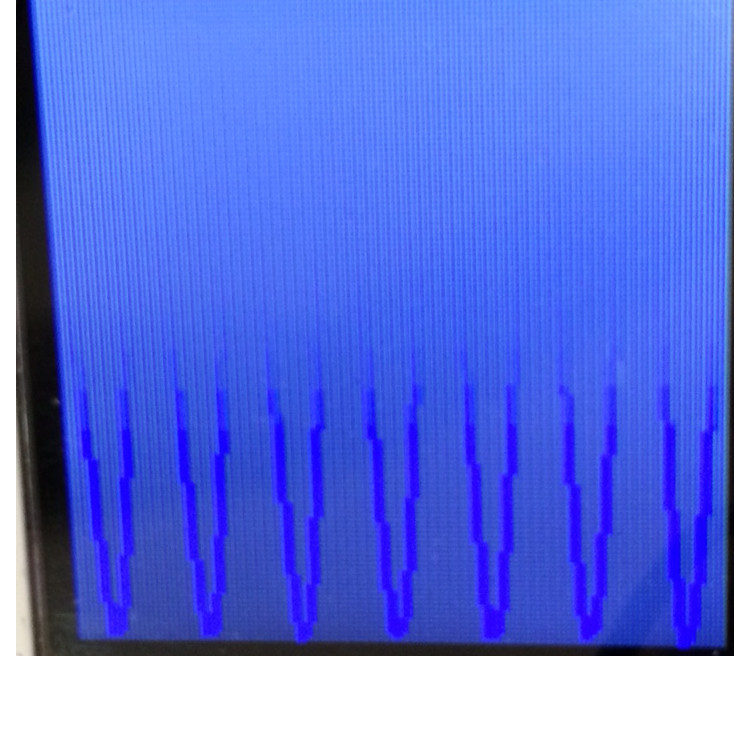
\includegraphics[width=\textwidth]{./img/raw_200Hz}
    \caption{200 Hz}
    \label{fig:raw_200}
  \end{subfigure}
  \begin{subfigure}[b]{0.3\textwidth}
    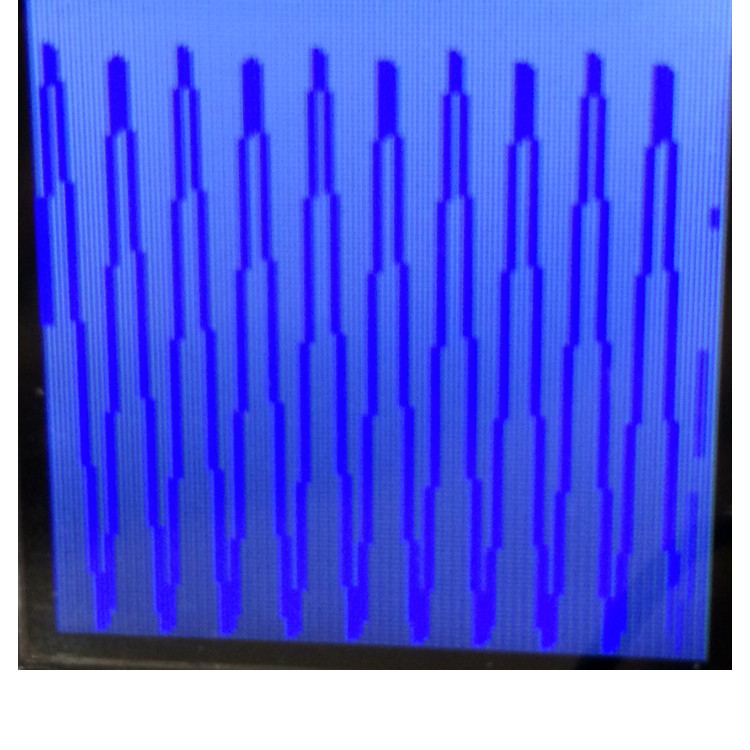
\includegraphics[width=\textwidth]{./img/raw_300Hz}
    \caption{300 Hz}
    \label{fig:raw_300}
  \end{subfigure}
  \begin{subfigure}[b]{0.3\textwidth}
    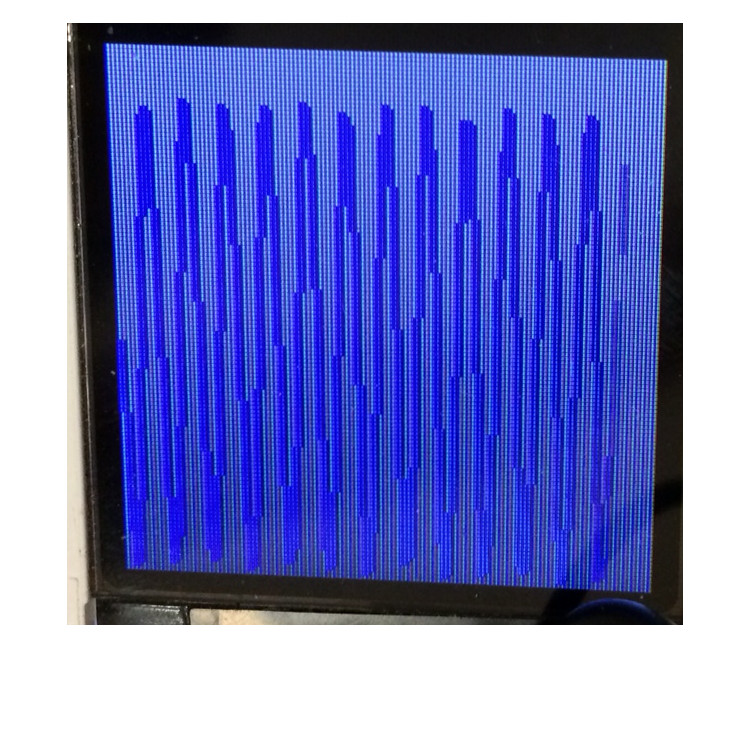
\includegraphics[width=\textwidth]{./img/raw_400Hz}
    \caption{400 Hz}
    \label{fig:raw_400}
  \end{subfigure}
  \begin{subfigure}[b]{0.3\textwidth}
    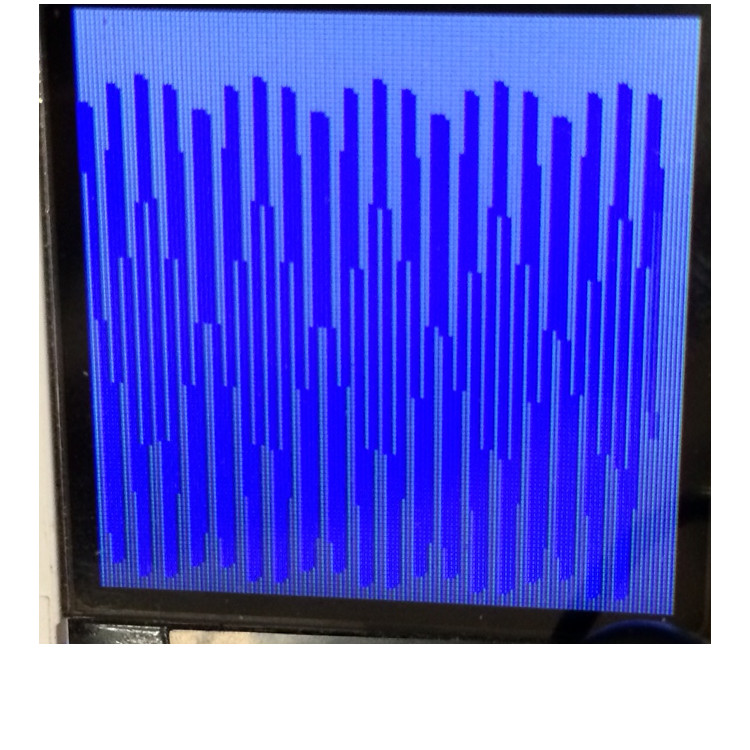
\includegraphics[width=\textwidth]{./img/raw_500Hz}
    \caption{500 Hz}
    \label{fig:raw_500}
  \end{subfigure}
  \caption{LCD plots of raw data}
  \label{fig:lcd-plots-raw}
\end{figure}

\begin{figure}[H]
  \centering
  \begin{subfigure}[b]{0.3\textwidth}
    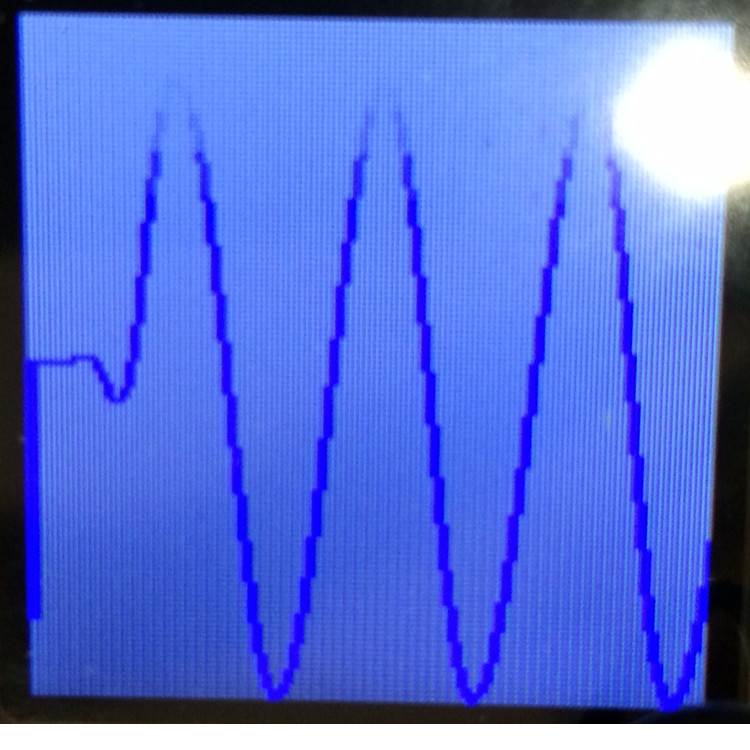
\includegraphics[width=\textwidth]{./img/filtered_100Hz}
    \caption{100 Hz}
    \label{fig:filtered_100}
  \end{subfigure}
  \begin{subfigure}[b]{0.3\textwidth}
    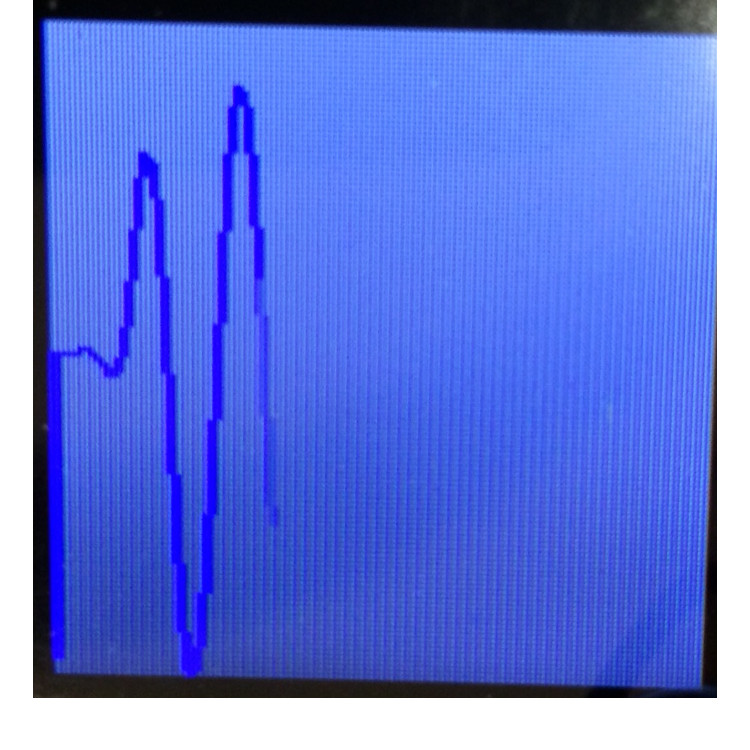
\includegraphics[width=\textwidth]{./img/filtered_200Hz}
    \caption{200 Hz}
    \label{fig:filtered_200}
  \end{subfigure}
  \begin{subfigure}[b]{0.3\textwidth}
    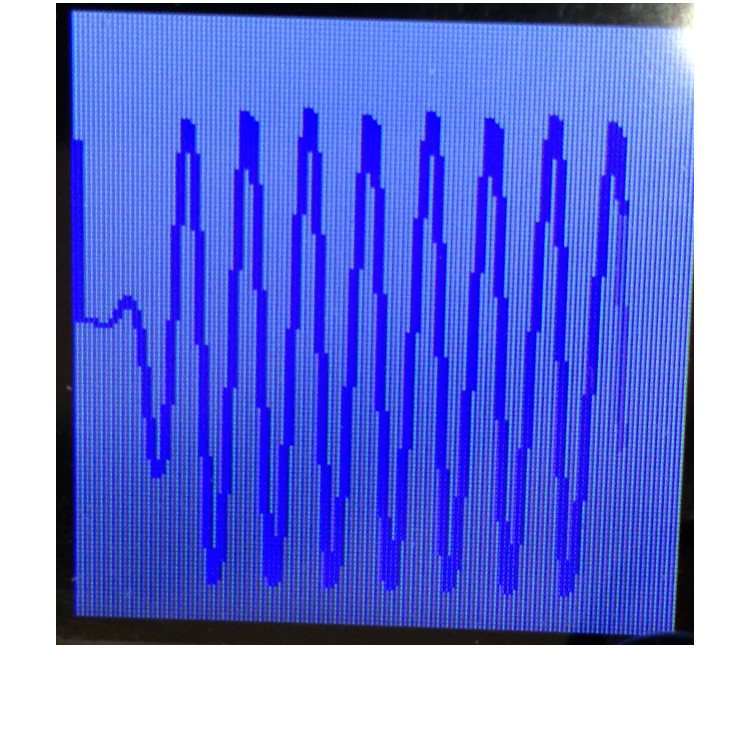
\includegraphics[width=\textwidth]{./img/filtered_300Hz}
    \caption{300 Hz}
    \label{fig:filtered_300}
  \end{subfigure}
  \begin{subfigure}[b]{0.3\textwidth}
    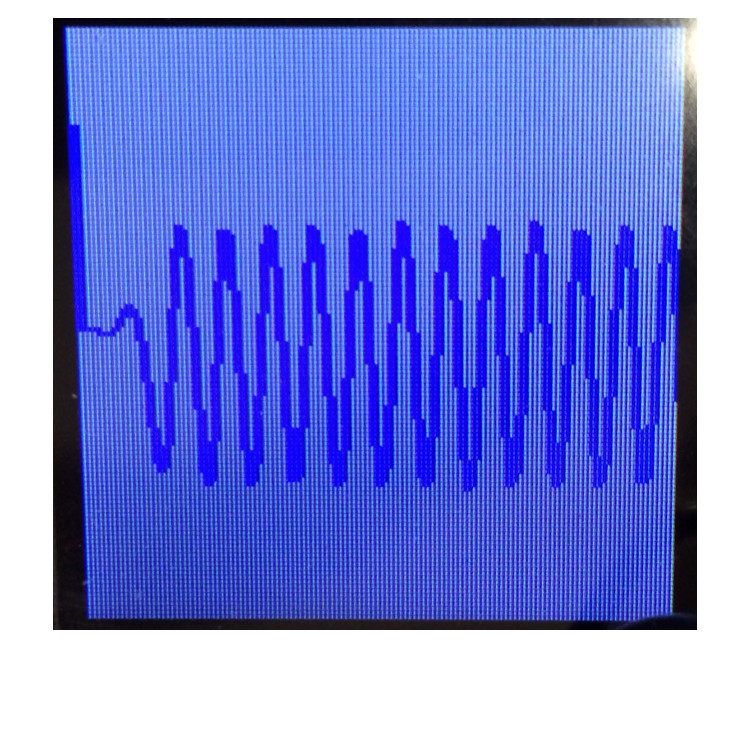
\includegraphics[width=\textwidth]{./img/filtered_400Hz}
    \caption{400 Hz}
    \label{fig:filtered_400}
  \end{subfigure}
  \begin{subfigure}[b]{0.3\textwidth}
    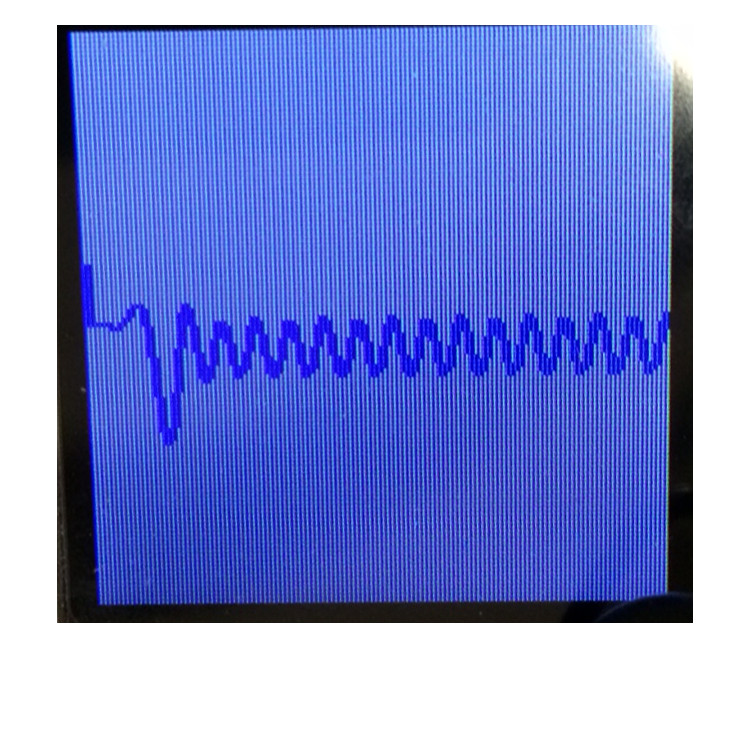
\includegraphics[width=\textwidth]{./img/filtered_500Hz}
    \caption{500 Hz}
    \label{fig:filtered_500}
  \end{subfigure}
  \begin{subfigure}[b]{0.3\textwidth}
    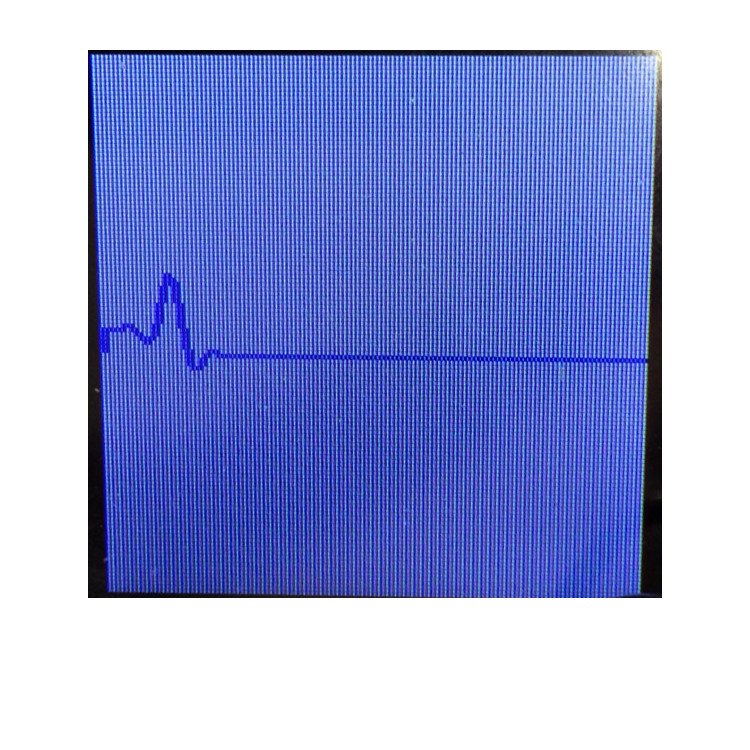
\includegraphics[width=\textwidth]{./img/filtered_600Hz}
    \caption{600 Hz}
    \label{fig:filtered_600}
  \end{subfigure}
  \caption{LCD plots utilizing the software low-pass filter}
  \label{fig:lcd-plots-filtered}
\end{figure}

\begin{figure}[H]
  \begin{subfigure}[b]{0.45\textwidth}
    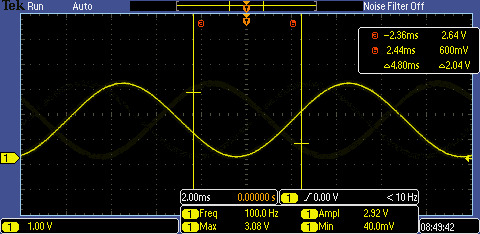
\includegraphics[width=\textwidth]{./img/TEK00002}
    \caption{100 Hz}
    \label{fig:dig_100}
  \end{subfigure}
  \begin{subfigure}[b]{0.45\textwidth}
    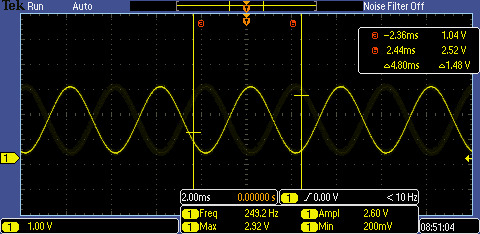
\includegraphics[width=\textwidth]{./img/TEK00003}
    \caption{250 Hz}
    \label{fig:dig_250}
  \end{subfigure}
  \begin{subfigure}[b]{0.45\textwidth}
    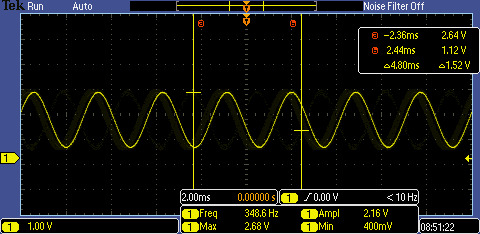
\includegraphics[width=\textwidth]{./img/TEK00004}
    \caption{350 Hz}
    \label{fig:dig_350}
  \end{subfigure}
  \begin{subfigure}[b]{0.45\textwidth}
    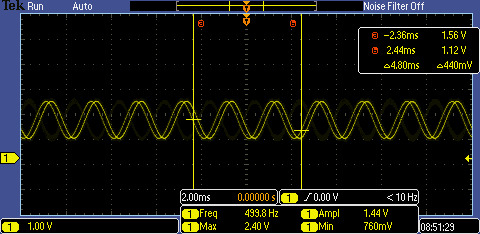
\includegraphics[width=\textwidth]{./img/TEK00005}
    \caption{500 Hz}
    \label{fig:dig_500}
  \end{subfigure}
  \begin{subfigure}[b]{0.45\textwidth}
    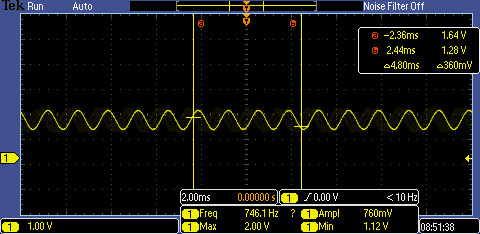
\includegraphics[width=\textwidth]{./img/TEK00006}
    \caption{750 Hz}
    \label{fig:dig_750}
  \end{subfigure}
  \begin{subfigure}[b]{0.45\textwidth}
    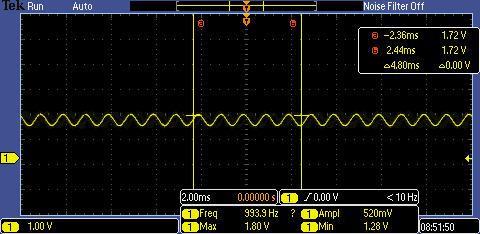
\includegraphics[width=\textwidth]{./img/TEK00007}
    \caption{940 Hz}
    \label{fig:dig_940}
  \end{subfigure}
  \begin{subfigure}[b]{0.45\textwidth}
    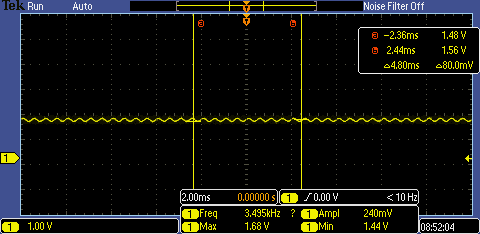
\includegraphics[width=\textwidth]{./img/TEK00008}
    \caption{3.5 KHz}
    \label{fig:dig_4000}
  \end{subfigure}
  \label{fig:oscope-plots}
  \caption{Oscilloscope plots of the hardware low-pass filter}
\end{figure}

\newpage
\section{Code}
\lstinputlisting[language=C,label=lst:lab4,caption=\texttt{lab4.c}]{@doc-staging-area@/lab4.c}
\lstinputlisting[language=Octave,label=lst:filtergen,caption=\texttt{filter\_gen.m}]{@doc-staging-area@/filter_gen.m}
\lstinputlisting[language=Octave,label=lst:signalgen,caption=\texttt{signal\_gen.m}]{@doc-staging-area@/signal_gen.m}
\lstinputlisting[language=Octave,label=lst:filtertest,caption=\texttt{filter\_test.m}]{@doc-staging-area@/test.m}

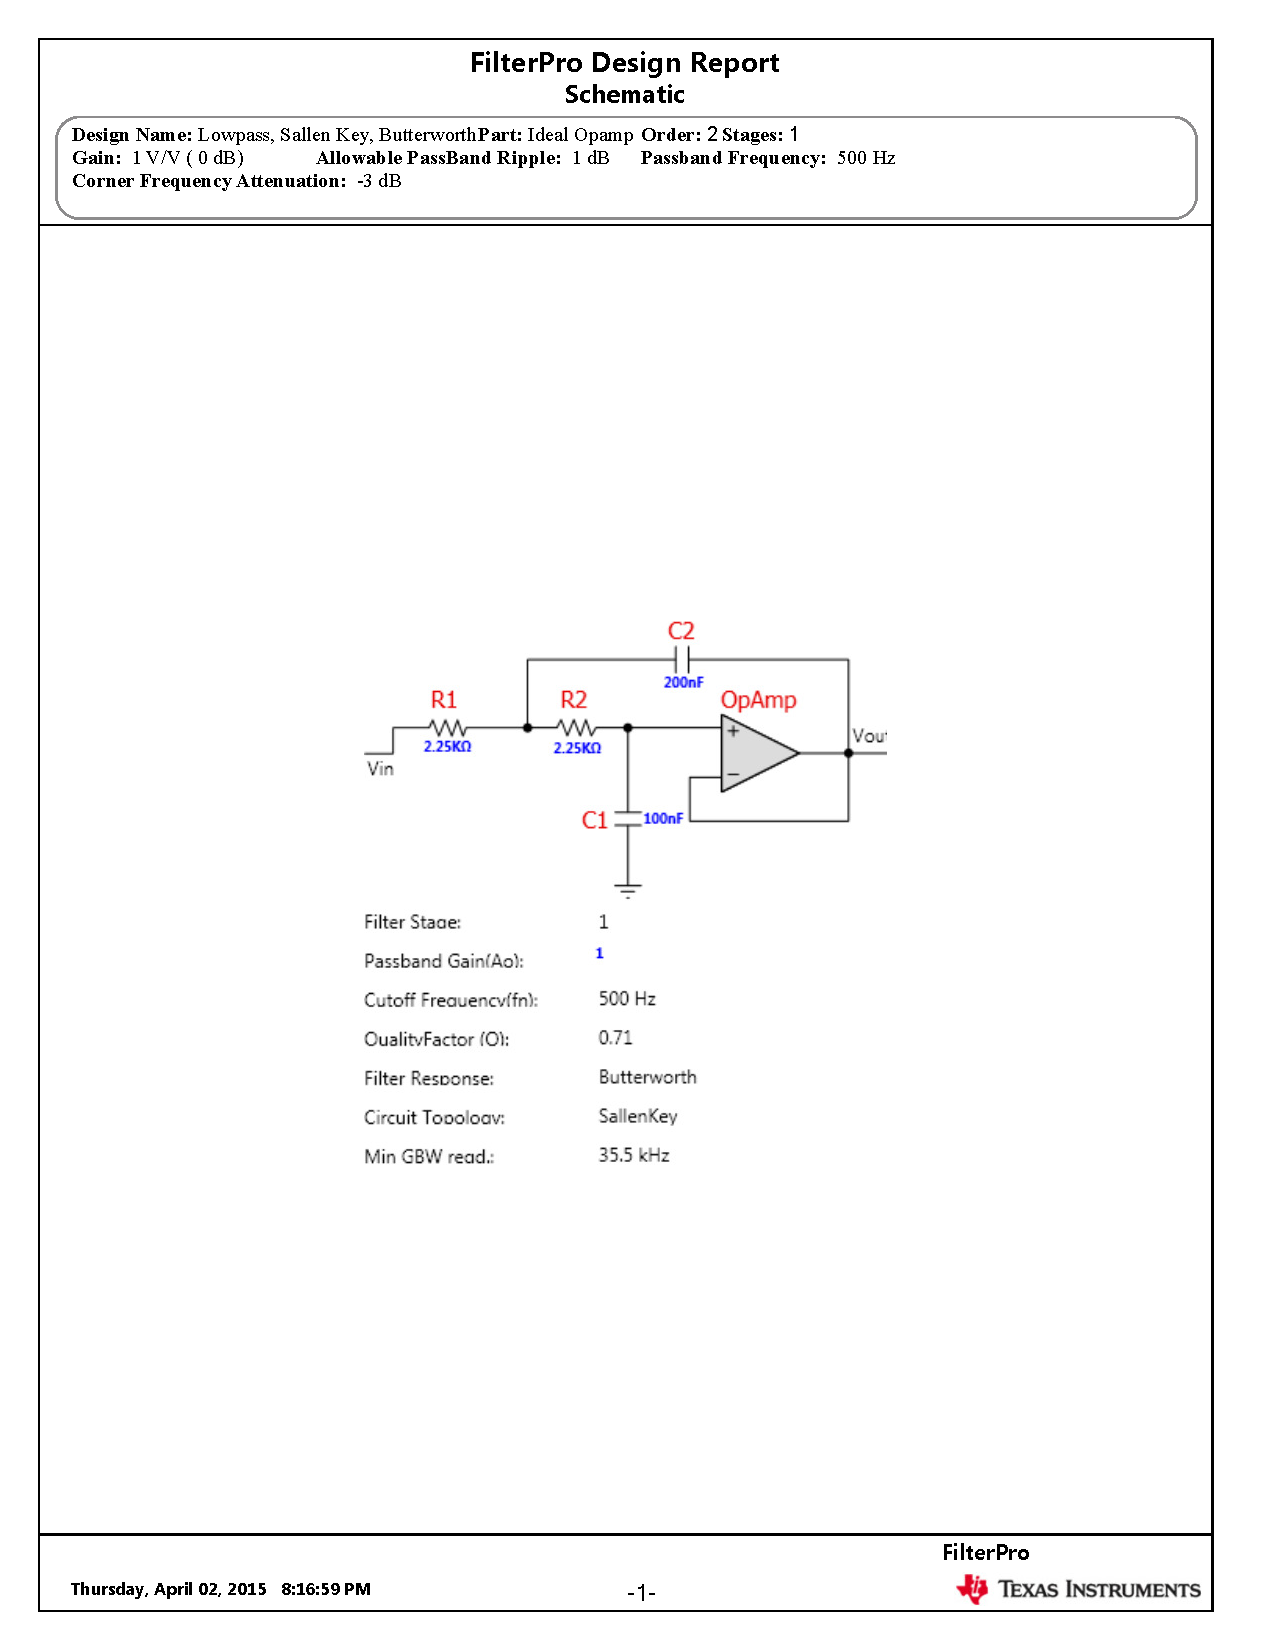
\includepdf[pages={1,2,3}]{./img/analog-filter-design.pdf}

\end{document}
